
\begin{abstract}
This demo paper accompanies an ESWC 2025 resource paper.
Authoring Semantic Web documents is error-prone, often leading to interoperability issues, validation failures, or incorrect reasoning. 
  To address these challenges, we present the Semantic Web Language Server (SWLS), a tool that integrates IDE-like functionalities such as real-time syntax validation, intelligent autocompletion, and SHACL-based diagnostics into modern code editors.
  SWLS follows the Language Server Protocol (LSP), allowing seamless integration with editors like Visual Studio Code and NeoVim while supporting multiple formats, including Turtle, SPARQL, and JSON-LD.
This demo showcases SWLS in an interactive web-based environment, where users can explore its features across four dedicated editor panes: an RDF data editor, an ontology editor, a SHACL constraint editor, and a SPARQL query editor.
  The demo highlights SWLS's ability to detect errors, suggest completions based on ontology imports, and assist users in writing correct and interoperable Semantic Web documents.
  By improving the development workflow and reducing common pitfalls, SWLS enhances the usability of Semantic Web technologies and facilitates broader adoption.
\keywords{Language Server, IDE, Tool, Linked Open Vocabularies, Semantic Web}
\end{abstract}

\textbf{URL:} \url{https://github.com/ajuvercr/semantic-web-lsp} 

\textbf{Licenses:} MIT License


\section{Introduction}%
\label{sec:introduction}

The Semantic Web comprises a variety of syntaxes for expressing and querying data, including Turtle, JSON-LD, and SPARQL. 
While these formats enable representing semi-structured data in an interoperable way, they are prone to human errors, which can lead to non-interoperability, validation failures or incorrect reasoning outcomes.
For instance, mistyping the URI of a prefix can alter the entire meaning of a document, rendering it non-interoperable with other datasets.

However, open services such as Linked Open Vocabularies (LOV)\cite{LOV2017} provide exact definitions of predicates and classes, offering a reliable reference for avoiding such errors.

In this paper, we introduce the \textbf{Semantic Web Language Server (SWLS)}, a language server designed to assist editors in handling semantic web documents.
This demo paper accompanies an ESWC 2025 resource paper.

SWLS is not the only software that introduces IDE-like functionalities for Semantic Web documents.
While tools such as YASGUI\cite{yasgui,10.1007/978-3-642-41242-4_7} and \href{https://query.wikidata.org/}{query.wikidata.org} provide robust web-based functionalities,
they do not integrate seamlessly into local development environments or support a broader range of Semantic Web formats.
In contrast, SWLS runs locally, allowing for quick development cycles and seamless integration into the developer's workflow. 
Moreover, SWLS supports multiple formats beyond Turtle it supports SPARQL and JSON-LD, making it a more versatile solution.

\section{Semantic Web Language Server}

SWLS follows the Language Server Protocol (LSP)\cite{IntroToLsp}\footnote{\url{https://microsoft.github.io/language-server-protocol/}},
a protocol designed by Microsoft to allow one server implementation to interact with different editors, reducing complexity from $O(M*N)$ to $O(M+N)$,
where $M$ is the number of existing editors and $N$ the number of supported language implementations.

The server communicates using JSON-RPC, enabling bidirectional messaging between the editor and server for handling features such as autocompletion, highlighting, and diagnostics.
Most modern editors support LSP, including Visual Studio Code and NeoVim.

SWLS is designed for flexibility, allowing support for multiple file formats with maximal code reuse. 
It uses an entity component system to build a layered architecture\cite{10.1145/3550355.3552452}, following a traditional \textit{Feature Execution Flow} with three steps.

\begin{enumerate}
  \item In the \textit{Parse} step of the server handles parsing the document (emitting potential syntax errors) and deriving defined triples and prefixes.

  \item The \textit{Traverse} step derives information from the triples, such as defined properties, classes and SHACL shapes. 
        This step also fetches the used ontologies that are accessable from the defined prefixes,
        this uses the public LOV api, when these documents are fetched they are added to the ECS.
        The \textit{Traverse} step also emits dignostics, notifying the editor of potential mistakes in the document. 
        These include undefined prefixes, or shape violations (using the Rudof\cite{labra2022rudof} library).

  \item The \textit{Process} step extracts all required information from the previous steps and translates it into a response for the current request.
        Currently SWLS handles autocompletion (predicates, classes and prefixes), renaming and hover.
\end{enumerate}
 
The ECS design enables reusing the systems for the \textit{Traverse} and \textit{Process} steps across different languages, 
requiring only the \textit{Parse} step to be implemented for each file format.

\section{Demo}

\begin{figure}[tb]
    \centering
    \begin{subfigure}{0.48\textwidth}
      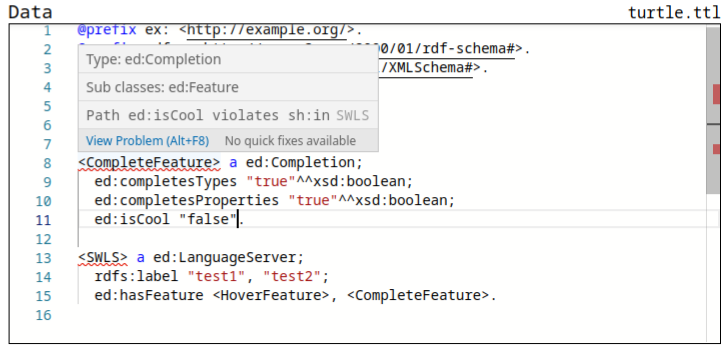
\includegraphics[width=\textwidth]{./images/hover.png}
      \caption{SWLS shows the user type information on hover as well as diagnostics}
      \label{hover}
    \end{subfigure}
    \hfill
    \begin{subfigure}{0.48\textwidth}
      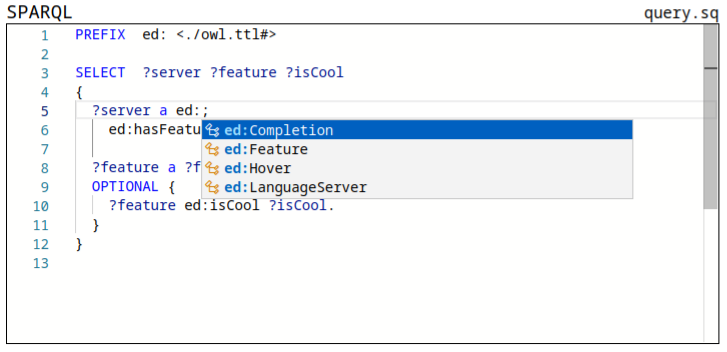
\includegraphics[width=\textwidth]{./images/class.png}
      \caption{SWLS completes a class when the user wants to write a class}
      \label{class_completion}
    \end{subfigure}
    \hfill
    \begin{subfigure}{0.48\textwidth}
      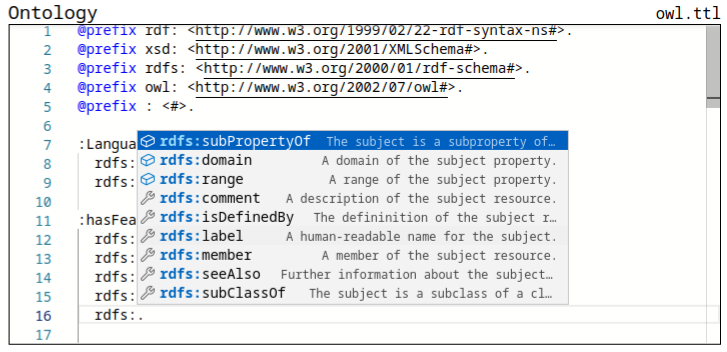
\includegraphics[width=\textwidth]{./images/property.png}
      \caption{SWLS completes properties, first the properties with the correct domain}
      \label{property_completion}
    \end{subfigure}
    \hfill
    \begin{subfigure}{0.48\textwidth}
      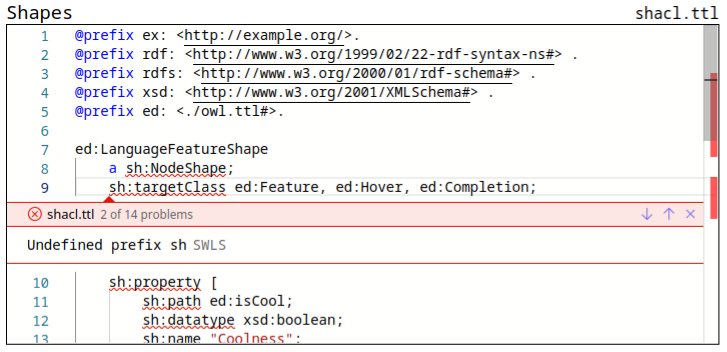
\includegraphics[width=\textwidth]{./images/undefined.png}
      \caption{SWLS notifies the user of undefined prefixes}
      \label{undefined_prefix}
    \end{subfigure}
    \caption{
      Demo application that shows the usage of SWLS. Features include hover information, autocompletion and diagnostics.
    }\label{lst:Demo}
\end{figure}

The demo consists of an online application at \url{https://ajuvercr.github.io/semantic-web-lsp/}.
The app has four editor panes each with a different purpose.
% : a data pane for authoring RDF data, an ontology pane for vocabulary management, a shape pane for SHACL constraints, and a query pane for SPARQL queries.
%
% All panes are treated equally, except for the query pane, which is designed for SPARQL rather than Turtle, but uses the same SWLS instance.

\begin{enumerate}
  \item The \textbf{data pane} presents an RDF dataset, where users can author and edit linked data.
    Errors detected via SHACL validation are highlighted, as shown in Figure \ref{hover}.
    Users can correct these errors either by adding missing triples or modifying the shape definitions in the shape pane.
  \item The \textbf{ontology pane} contains a playground ontology that describes language servers.
    It is linked to the data pane using a prefix import, enabling autocompletion of relevant properties, as shown in Figure \ref{property_completion}.
  \item The \textbf{query pane} allows users to write SPARQL queries against the data. 
    While SWLS does not execute queries, it provides autocompletion for classes and properties, as depicted in Figure \ref{class_completion}.
  \item The \textbf{shape pane} includes SHACL constraints imported into the data pane via the \texttt{owl:imports} property. 
    As shown in Figure \ref{undefined_prefix}, SWLS alerts users to undefined prefixes, and typing a prefix triggers autocompletion suggestions, adding the import statement.
\end{enumerate}

Users can also try the language server on local editors.
For VSCodes, users can install the Semantic Web LSP\footnote{\url{https://marketplace.visualstudio.com/items?itemName=ajuvercr.semantic-web-lsp}}.
Seting the server up  with NeoVim requires installing the language server with cargo and configuring the language server with \textit{lspconfig}.

\section{Conclusion}

The Semantic Web Language Server (SWLS) introduces IDE-like functionalities for authoring Semantic Web documents, supporting multiple formats and providing a local development workflow. 
By integrating features such as real-time validation, context-aware autocompletion, and SHACL-based diagnostics, SWLS lowers the chance of errors in local documents.
Unlike existing tools, SWLS runs locally and extends beyond Turtle, offering a more flexible and powerful authoring experience.
This work not only addresses current limitations in Semantic Web tooling but also paves the way for broader adoption of semantic technologies by reducing barriers and improving usability.


